
\documentclass[a4paper,11pt]{exam}
\usepackage{color}
\usepackage[francais]{babel}
\usepackage{graphicx}
\usepackage[utf8]{inputenc}
\usepackage{eurosym}
\usepackage{xcolor}
\usepackage[formats]{listings}
\usepackage{hyperref}
\usepackage{comment}

\usepackage{listings, xcolor}

\newcommand{\nadjib}[2][Nadjib]
{$^{\fboxsep=1pt\fbox{\tiny #1}}$%
	\marginpar{\fbox{\parbox[t]{\marginparwidth}{\tiny #2}}}}
\lstset{language=Java,
	basicstyle=\ttfamily,
	keywordstyle=\color{javapurple}\bfseries,
	stringstyle=\color{javared},
	commentstyle=\color{javagreen},
	morecomment=[s][\color{javadocblue}]{/**}{*/},
	numbers=left,
	numberstyle=\tiny\color{black},
	stepnumber=2,
	numbersep=10pt,
	tabsize=4,
	showspaces=false,
	showstringspaces=false}
\definecolor{dkgreen}{rgb}{0,0.6,0}
\definecolor{gray}{rgb}{0.5,0.5,0.5}
\definecolor{mauve}{RGB}{114,18,82}
\definecolor{mauve2}{rgb}{0.58,0,0.82}


\usepackage{wrapfig}
%\usepackage{../feuilleExos}

\usepackage[a4paper,bindingoffset=0.2in,%
            left=1.5cm,right=2.3cm,top=2cm,bottom=2.2cm]{geometry}%~ 
\hypersetup{
    unicode=false,          % non-Latin characters in Acrobats bookmarks
    pdftoolbar=true,        % show Acrobats toolbar?
    pdfmenubar=true,        % show Acrobats menu?
    pdffitwindow=true,      % page fit to window when opened
    pdftitle={TD1},    % title
    pdfauthor={Author},     % author
    pdfsubject={Subject},   % subject of the document
    pdfcreator={Creator},   % creator of the document
    pdfproducer={Producer}, % producer of the document
    pdfkeywords={keywords}, % list of keywords
    pdfnewwindow=true,      % links in new window
    colorlinks=true,       % false: boxed links; true: colored links
%    linkcolor=blue!75!black,          % color of internal links
    citecolor=blue,        % color of links to bibliography
    filecolor=magenta,      % color of file links
    urlcolor=blue           % color of external links
}
\usepackage{changepage}

\newcommand{\point}{$\bullet$\ }

\def\JAVA{\mintinline[escapeinside=||]{java}}
\def\String{{\tt String}}
\def\int{{\tt int}}
\def\float{{\tt float}}
\def\ra{$\rightarrow$~}


\lstdefineformat{Java}
{
  \{=\string\newline\indent,%
  \}=\newline\noindent\string\newline,%
  ;=[\ ]\string\space,%
}



\lstset{
  language=Java,
  aboveskip=3mm,
  belowskip=3mm,
  showtabs=false,
  showspaces=false,
  showstringspaces=false,
  columns=fullflexible,
  basicstyle={\ttfamily},
  numbers=none,
  numberstyle=\tiny\color{gray},
  keywordstyle=\bfseries\color{blue},
  commentstyle=\color{dkgreen},
  stringstyle=\color{mauve2},
  identifierstyle=\ttfamily,
  breaklines=true,
  breakatwhitespace=true,
  tabsize=3,
  extendedchars=true,
  literate={é}{{\'e}}1
           {è}{{\`e}}1
           {à}{{\`a }}1
           {ê}{{\^e}}1
           {î}{{\^i}}1
}

% ====== Feuille enseignant (AVEC) les corrections :
 \includecomment{comment}
 \includecomment{suggestion}
%%% ====== Feuille etudiants (SANS) les corrections :
%\excludecomment{comment}
%\excludecomment{suggestion}


\newcommand{\titre}[1]{
	
	\ \hfill {\bf\large #1} \hfill \ 
	% \vspace{.5em}
}


\begin{document}

\pagestyle{plain}

{\noindent
	\textit{R3.04 - Qualité de développement}
	\hfill \textit{IUT Montpellier-Sète}\\
}
{\noindent \textit{Année 2022-2023}
	\hfill \textit{Département Informatique}\\
}
{\noindent \textit{--$\qquad\qquad\qquad$}
	\textbf{M. Gasquet, G. Hisler, N. Lazaar, N. Palleja, S. Robillard, B. Rouchon}\\
}
\vspace*{-0.3cm}
\hrule



%\noindent
%~\hrulefill~

\begin{comment}
\titre{VERSION ENSEIGNANT}
\newline
\end{comment}

\vspace*{1.5cm}
  
\begin{center}
	\huge{\textbf{{Les patrons Décorateur et Adaptateur}}}\\
\end{center}

\newcounter{exo}
%\newcounter{question}
\setcounter{exo}{0}
\setcounter{question}{0}

\begin{comment}
\vspace{5ex}
\stepcounter{exo}
\noindent\fbox{\large{\textbf{\textsf{Exercice \theexo}}}}
\medskip
\end{comment}

\vspace*{0.5cm}

\section{Partie UML}
Au cours de cet exercice, nous allons construire un diagramme de classe incrémentalement. Chacune des questions enrichira donc celui-ci.
Pour chaque classe, indiquer ses attributs (privés), ses opérations (incluant la redéfinition de la méthode \texttt{toString()}), et son ou ses constructeurs. 

On souhaite gérer un banc de test pour étudier les performances de divers composants de voitures. \\
Une voiture est constituée d'un châssis, d'un ou plusieurs moteurs, d'un ou plusieurs types de freins,...


\paragraph*{\textsf{Question \thequestion}}\ 
\point On imagine que les voitures peuvent être montées avec toute combinaison de composants comme des moteurs à essence, des moteurs diesel, des moteurs électriques, des freins à disque, et toutes sortes de composants de voiture à l'infini...\\
A quoi pourrait ressembler un premier diagramme de classes modélisant toutes ces voitures ? 

\stepcounter{question} 
\paragraph*{\textsf{Question \thequestion}}\ 
\point Définissez l'interface \textbf{Voiture}, comprenant des accesseurs pour une accélération (\float), un freinage (\float), une masse (\float) et pour un prix (\float).
\stepcounter{question} 
\paragraph*{\textsf{Question \thequestion}}\ 
\point Ajoutez au diagramme de classes une implémentation de cette interface nommée \textbf{Chassis} (sans oublier les attributs). \\\\


Comme l'objectif du banc est de tester les diverses combinaisons d'options, vous allez utiliser le patron \emph{Décorateur} et monter la voiture comme un mécano.

\subsection{Le décorateur}


\stepcounter{question} 
\paragraph*{\textsf{Question \thequestion}}\ 
\point Complétez le diagramme en définissant une classe abstraite \textbf{VoitureMontee}, qui applique le patron en enveloppant une voiture.

\stepcounter{question} 
\paragraph*{\textsf{Question \thequestion}}\ 
\point Définissez ensuite les classes \textbf{VoitureMoteurEssence} et \textbf{VoitureMoteurDiesel} qui modifient les méthodes
\texttt{getAcceleration()}, \texttt{getFreinage()}, \texttt{getMasse()} et \texttt{getPrix()}.

\stepcounter{question} 
\paragraph*{\textsf{Question \thequestion}}\ 
\point Donnez le code Java de la méthode \texttt{getMasse()} de \textbf{VoitureMoteurEssence} en supposant que le moteur pèse 300~Kg.


\begin{comment}
\begin{lstlisting}[language = Java , frame = trBL , firstnumber = last , escapeinside={(*@}{@*)}]
@Override
public float getMasse() {
return voiture.getMasse() + 300; // Retourne la masse de la voiture encapsulée augmentée de 300 Kg
}                                
\end{lstlisting}
	
\end{comment}

\stepcounter{question} 
\paragraph*{\textsf{Question \thequestion}}\ 
\point De manière similaire, ajoutez les classes \textbf{VoitureFreinsDisque} et \textbf{VoitureFreinsFoucault} qui modifieront la force de freinage. Détaillez le code des différentes méthodes.\\
Vous pouvez constater maintenant que, afin de respecter le principe DRY, votre code peut être "refactorer" en extrayant une partie vers la classe (abstraite) de base.

\begin{comment}
\begin{lstlisting}[language = Java , frame = trBL , firstnumber = last , escapeinside={(*@}{@*)}]
// méthode dans la classe VoitureMontee
public float getMasse() {
return voiture.getMasse();
}
@Override
public float getMasse() {
return super.getMasse() + 300; // Retourne la masse de la voiture encapsulée augmentée de 300 Kg
}                                
\end{lstlisting}
\end{comment}

\stepcounter{question} 
\paragraph*{\textsf{Question \thequestion}}\ 
\point Donnez le code des constructeurs des \textbf{VoitureMontee} et \textbf{VoitureMoteurEssence}, puis celui permettant d'instancier une voiture hybride avec un moteur essence, un moteur diesel et des freins à disque.
\begin{comment}
\begin{lstlisting}[language = Java , frame = trBL , firstnumber = last , escapeinside={(*@}{@*)}]
// constructeur dans la classe VoitureMontee
public VoitureMonte(Voiture voiture) {
this.voiture = voiture;
}
// constructeur dans les dérivées
public VoitureMoteurEssence(Voiture voiture) {
super(voiture);
}                             
// construction de la voiture hybride
Voiture uneVoitureHybride = new VoitureMoteurEssence( new VoitureMoteurDiesel ( new VoitureFreinsDisque (new Chassis() ) ) );
\end{lstlisting}
\end{comment}


\subsection{L'adaptateur}
Le \textbf{BancDeTest} remplit une fiche de renseignements pour chaque voiture, et sa méthode \texttt{lancerTests()} retourne la liste des fiches remplies.

\stepcounter{question} 
\paragraph*{\textsf{Question \thequestion}}\ 
\point Ajoutez au diagramme une classe \textbf{Fiche} contenant des données telles que la voiture concernée, sa vitesse maximale ou sa distance de freinage. On ne notera pas les accesseurs/mutateurs par souci d'économie.\\

On aimerait maintenant trier notre liste de fiches selon divers critères, choisis à l'exécution. En java, la méthode statique {\tt Collections.sort} permet le tri d'une liste, à condition que les éléments soient {\tt Comparable}. 

\stepcounter{question} 
\paragraph*{\textsf{Question \thequestion}}\ 
\point Ajoutez au diagramme UML une classe \textbf{TriFicheVitesse} qui servira d'\emph{adaptateur} entre une \textbf{Fiche} et l'interface {\tt Comparable <TriFicheVitesse>}. Elle devra en particulier définir la méthode {\tt compareTo(TriFicheVitesse autre)} qui retourne un entier -1, 0 ou +1 selon l'ordre des fiches comparées.\\

On considère maintenant des chassis fabriqués par un consortium européen que l'on doit pouvoir monter dans toute voiture et tester sur notre banc d'essai. La classe \textbf{ChassisEuropeen} est fournie, elle possède exactement les mêmes méthodes que l'interface Voiture. Cependant, cette classe étant fournie sous sa version compilée, il n'est absolument pas possible de la modifier.
\stepcounter{question} 
\paragraph*{\textsf{Question \thequestion}}\
\point Comment peut-on utiliser ce chassis dans une voiture ? Donnez le diagramme de classes, puis détaillez le code.\\
\begin{comment}
\begin{lstlisting}[language = Java , frame = trBL , firstnumber = last , escapeinside={(*@}{@*)}]
Ici on ne peut pas ajouter implements Voiture à la classe existante, donc il faut créer une nouvelle classe avec un "héritage multiple"
\end{lstlisting}
\end{comment}

On considère ensuite des \textbf{ChassisAnglais} fabriqués au Royaume Uni, et pour lesquels une classe (ici encore non modifiable) est fournie, mais dont les identificateurs de méthodes sont en anglais \texttt{getMass}, \texttt{getBraking}, \texttt{getPrice}...

\stepcounter{question} 
\paragraph*{\textsf{Question \thequestion}}\
\point Proposez une solution permettant d'utiliser ce chassis dans une voiture, puis détaillez le code du constructeur et de l'accesseur pour la masse.
\begin{comment}
\begin{lstlisting}[language = Java , frame = trBL , firstnumber = last , escapeinside={(*@}{@*)}]
Il faut cette fois utiliser la délégation puisque, les méthodes ne portant pas le même nom, on veut exactement le même jeu de méthodes que l'interface à implémenter et pas plus.
\end{lstlisting}
\end{comment}

\newpage
\begin{comment}
	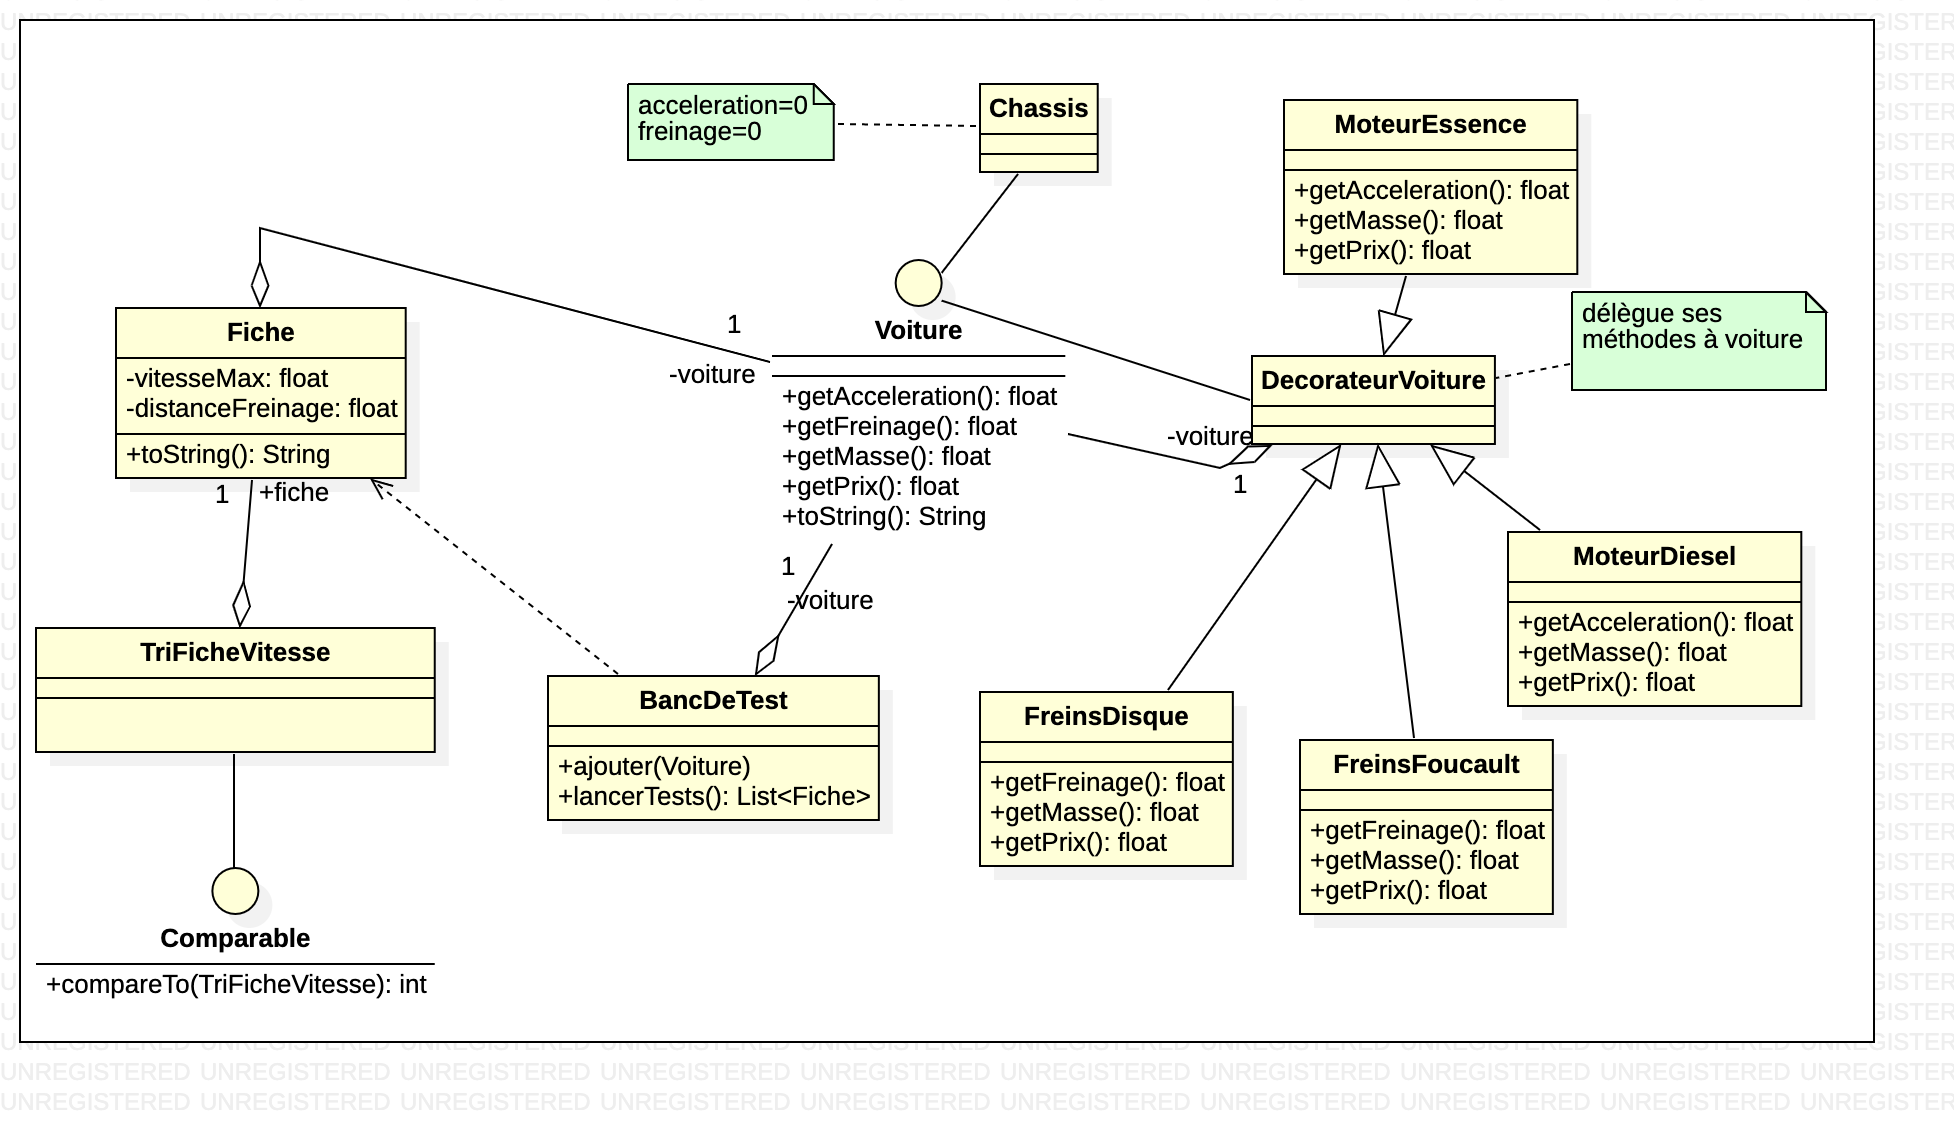
\includegraphics[scale=0.25]{./uml/VOITURE.png}
\end{comment}
\section{Partie Java}

L'objectif de cette partie est d'implanter et de tester les différents diagrammes que vous avez réalisés dans la première partie du TD. N'attendez pas d'avoir tout écrit pour tester !

Dans votre dépôt local, vous trouverez l'interface {\tt Voiture}, qui est un peu plus riche que celle vue dans la partie UML, et les classes {\tt Chassis}, {\tt FreinDisque}, {\tt FreinFoucault}, {\tt MoteurDiesel}, {\tt MoteurEssence}, {\tt Fiche} et {\tt DynamiqueVoiture}. Cette dernière s'occupe de tous les calculs du banc de test.

\stepcounter{question} 
\paragraph*{\textsf{Question \thequestion}}\ 
\point Ajoutez la classe abstraite {\tt VoitureMontee} qui implémente l'interface {\tt Voiture}. 

\stepcounter{question} 
\paragraph*{\textsf{Question \thequestion}}\ 
\point Connectez les sous-classes {\tt FreinDisque}, {\tt FreinFoucault}, {\tt VoitureMoteurDiesel}, {\tt VoitureMoteurEssence} à la super-classe {\tt VoitureMontee} (héritage).
Sachant que la masse, la puissance et le coefficient de freinage sont cumulables, n'oubliez pas de redéfinir les méthodes au niveau des sous-classes.

\stepcounter{question} 
\paragraph*{\textsf{Question \thequestion}}\ 
\point Dans la fonction {\tt main}  de la classe {\tt BancDeTest}, construisez et ajoutez une voiture dotée d'un châssis, d'un moteur, et d'un système de freins.
Ajoutez la voiture au banc de test et lancez les tests

\stepcounter{question} 
\paragraph*{\textsf{Question \thequestion}}\ 
\point Décorer maintenant avec différent composants vos voitures et admirez la force du patron.

\stepcounter{question} 
\paragraph*{\textsf{Question \thequestion}}\ 
\point Ajoutez votre adaptateur {\tt TriFicheVitesse}.\\

%Il existe une solution plus simple pour le tri. Java vous propose l'interface {\tt Comparator<T>} qui possède une méthode {\tt compare(T o1, T o2) : int }. Celle-ci permet de jouer le rôle d'un ``adaptateur flottant'', le même adaptateur passant d'élément en élément... 

Vous pouvez ainsi trier votre liste en utilisant :

\begin{lstlisting}[language = Java , frame = trBL , firstnumber = last , escapeinside={(*@}{@*)}]
Collections.sort(resultats, (ficheResultat, autre) -> ficheResultat.compareAcceleration(autre));

\end{lstlisting}

Ou encore, avec une référence de méthode (Java 8+) :

\begin{lstlisting}[language = Java , frame = trBL , firstnumber = last , escapeinside={(*@}{@*)}]

Collections.sort(resultats, FicheResultat::compareAcceleration);

\end{lstlisting}

\end{document}
